\section{P e NP}

In questo capitolo cercheremo di esaminare un po' più in dettaglio le classi di complessità $\mathcal{P}$ e $\mathcal{NP}$, studiandone seppur superficialmente la struttura.\
Lo strumento principale che useremo, se non l'unico, è la ricerca di uno o più problemi completi per ciascuna di tali classi, cioè quei problemi che vi appartengono e di questa sono i più ardui, ovvero son tali per cui a loro si riducono tutti gli altri problemi della classe.\
Più precisamente, considereremo la relazione di riduzioni $\leqslant_{\mathrm{logspace}}$, cioè la relazione che impiega riduzioni, o algoritmi, di complessità $\mathrm{LOGSPACE} = \bigcup_{k\geq 1} \mathrm{SPACE}(k \times \log n)$, la quale classifica $\mathcal{P}$ e $\mathcal{NP}$, andremo poi a cercare problemi $H$ che siano $\mathcal{P}$-completi, cioè tali per cui ogni problema $I$ in $\mathcal{P}$ si riduce a $H$ (cioè $H$ è arduo) e inoltre $H$ appartiene a $\mathcal{P}$ (cioè $H$ è completo) (si veda la definizione \ref{rec_enumerabile}); analogamente per $\mathcal{NP}$.

I problemi completi caratterizzano davvero una classe di complessità, perché ne esprimono la struttura profonda e l'essenza e la difficoltà dei suoi problemi.\
Di conseguenza attraverso un problema completo si esprime anche il potere espressivo di una classe.\
A questo proposito, si ricordi l'insieme $K$ che è $RE$-completo per riduzioni calcolabili totali (così come lo sono $K_0$ e $K_1$) e il ruolo che esso gioca nel determinare i gradi di solubilità e insolubilità.\
Inoltre, sia detto per inciso, vale poco una classe che non ha problemi completi \textit{pre-esistenti} alla sua definizione e che siano interessanti dal punto di vista computazionale.\
Vedremo in questo capitolo alcuni problemi completi per $\mathcal{P}$ e per $\mathcal{NP}$, i quali sono davvero interesssanti e che son stati posti ben prima che nascesse la teoria della complessità come la conosciamo ora.\
Per ritornare sull'analogia con le classi di problemi calcolabili e di problemi non calcolabili, notiamo che l'insieme $K_0$ è davvero interessante:\ vorremmo, anche se da questa ricerca ne usciamo frustrati, uno strumento che dica, per ogni programma, se esso terminerà sempre --- in altre parole stiamo dichiarando che l'Entscheidungproblem proposto da Hilbert nel 1900 è interessante.\

\medskip
\noindent Prima di procedere, ricordiamo anche che si può stabilire il seguente frammento di gerarchia tra le classi di complessità che andremo a esaminare:
\[\mathrm{LOGSPACE} \subseteq \mathcal{P} \subseteq \mathcal{NP} \subseteq \mathrm{PSPACE} = \mathrm{NPSPACE}\]
e ricordiamo anche che $\mathrm{LOGSPACE} \subsetneq \mathrm{PSPACE}$.\
Di conseguenza, almeno una delle inclusioni
\[\mathrm{LOGSPACE} \subseteq \mathcal{P},\ \mathcal{P} \subseteq \mathcal{NP},\ \mathcal{NP} \subseteq \mathrm{PSPACE}\]
deve essere stretta.\
A tutt'oggi però non sappiamo quale essa sia, e non ci aiuta sapere anche che
\[\mathcal{P} \subsetneq \mathrm{EXP}\quad \mathrm{e} \quad \mathcal{NP} \subseteq \mathrm{EXP}\]
Il problema più interessante in questo momento è risolvere $\mathcal{P} \stackrel{?}{=} \mathcal{NP}$, che, oltre che estremamente affascinante si è rivelato resistentissimo, tanto che non si sa neppure se sia dimostrabile.\
Naturalmente, se facessimo vedere che un problema $\mathcal{NP}$-completo è risolto da un algoritmo che richiede tempo polinomiale deterministico, o che esso si riduce a un problema, necessariamente completo, che sta in $\mathcal{P}$, avremmo d'un botto dimostrato l'eguaglianza tra la classe dei problemi ``trattabili'' e dei problemi che divengono tali grazie al non determinismo (in accordo al paradigma:\ scommetti su una soluzione e dimostra che lo è in tempo polinomiale deterministico).\
Vi è tuttavia una sensazione diffusa che l'eguaglianza non valga, a ciò concorrono molti indizi.\
Tra questi segnaliamo soltanto il fatto che, se $\mathcal{P}$ coincidesse con $\mathcal{NP}$ ci sarebbe un modo computazionalmente accettabile di realizzare il meccanismo del non determinismo, cosa che appare per ora non poco sorprendente; a questo proposito si veda anche la nota a pagina 79 su due modelli di calcolo che paiono raggiungere tale obiettivo.\

Prima di iniziare discutiamo brevemente la robustezza delle classi $\mathcal{P}$ e $\mathcal{NP}$ e poi vediamo alcune critiche alla scelta di costruire una teoria asintotica che considera sempre il caso pessimo, e come queste si riverberano sulla tesi di Cook-Karp.\

\subsection{Problemi trattabili e intrattabili}

Adesso che abbiamo le nozioni di $\mathcal{P}$ e $\mathcal{NP}$ e che abbiamo visto come operano le macchine di Turing non deterministiche, possiamo rivedere l'affermazione che i problemi in $\mathcal{P}$ sono \textit{trattabili} e quelli in $\mathcal{NP}$ \textit{intrattabili}, ovvero discutiamo della fondatezza della \textit{tesi di Cook-Karp}.

A sostegno di questa tesi vi è la robustezza delle classi che stiamo considerando non solo rispetto alla rappresentazione dei dati e dei problemi, ma anche rispetto al cambio dei modelli di calcolo e di trasformazioni ``facili'' dei problemi stessi; vediamo in un dettaglio appena maggiore di quanto fatto che cosa intendiamo con le ultime due cose.\
\begin{itemize}
    \item[i)] Le classi $\mathcal{P}$ e $\mathcal{NP}$ sono robuste nel senso che non variano al variare dei modelli di calcolo, a patto che le funzioni per misurare il tempo siano ``ragionevoli''.\
          In altre parole $\mathcal{P}$ è robusta perché è chiusa rispetto la composizione polinomiale sinistra.\footnote{Una classe $\mathcal{C}$ di funzioni è chiusa rispetto la composizione polinomiale sinistra se per tutti i polinomi $p$ il fatto che $f \in \mathcal{C}$ implica $p \circ f \in \mathcal{C}$.}
          L'idea qui è che si può sempre trovare un algoritmo $T$ di complessità $p$ che, dato un problema $I$, \textit{trasforma} una sua procedura di decisione $M$, espressa in un modello $\mathcal{M}$, in una sua procedura \textit{equivalente} $P$, espressa in un altro modello $\mathcal{M}'$.\
          Se $M$ ha complessità polinomiale $f$, allora $P$ avrà complessità $p \circ f$, che è ancora un polinomio.\
          In termini più generali, robustezza rispetto al cambio di modelli di calcolo significa che le trasformazioni tra essi sono polinomiali (ad esempio, si consideri come un programma \textit{\footnotesize WHILE} può simulare in tempo polinomiale una macchina di Turing).
    \item[ii)]  La classe $\mathcal{P}$ è chiusa rispetto alla somma, al prodotto, alle riduzioni $\leqslant_F$ con $F$ (sotto-)classe dei polinomi.\
          Questo verrà formalizzato definendo appropriate riduzioni che classificano $\mathcal{P}$ e $\mathcal{NP}$ e dimostrando il teorema \ref{class_logspace}.\
          Per amore di simmetria rispetto quanto fatto sopra, ciò si può rifrasare prendendo riduzioni polinomiali e dicendo che $\mathcal{P}$ è chiusa rispetto alla composizione polinomiale destra.\
          \footnote{Una classe $\mathcal{C}$ di funzioni è chiusa rispetto la composizione polinomiale destra se per tutti i polinomi $p$, $f \in \mathcal{C}$ implica $f \circ p \in \mathcal{C}$.}
          In altre parole, per risolvere un problema $I$, trasformalo ``facilmente'', ovvero \textit{riducilo}, per mezzo di un algoritmo $M$, che ha come complessità un polinomio $p$, in $I' = M(I)$ e decidi $I'$; se $I' \in P$, cioè $I'$ è deciso in tempo deterministico polinomiale $f$, anche $I \in P$ perché è deciso in tempo deterministico $f \circ p$, che è ancora un polinomio.\

\end{itemize}

\noindent Un'ulteriore difesa della tesi di Cook-Karp è che di solito gli algoritmi polinomiali hanno, o almeno se ne cercano in modo che, le costanti moltiplicative e soprattutto gli esponenti siano piccoli, mentre gli algoritmi esponenziali diventano rapidamente inefficienti al crescere dei dati di ingresso.\

Tuttavia ci sono alcune critiche all'identificazione di $\mathcal{P}$ con i problemi trattabili:
\begin{itemize}
    \item[i)] Un algoritmo in $\mathcal{O}\left(n^{100}\right)$ non è certo efficiente.\ Lo è molto di più, almeno per $n$ non enormi, uno in $\mathcal{O}\left(2^{\frac{n}{100}}\right)$ o in $\mathcal{O}(n\log n)$.
    \item[ii)] Ci sono algoritmi che richiedono tempo esponenziale nel caso pessimo, ma sono efficienti nei casi interessanti o almeno in quelli più comuni.\ Si possono trovare degli esempi di questo comportamento bizzarro in:
          \begin{itemize}
              \item \textit{programmazione lineare}:\ l'algoritmo del simplesso è semplice e intuitivo e, benché sia esponenziale nel caso pessimo, di solito è efficiente, mentre il metodo elissoide è polinomiale, ma incredibilmente lento a causa di costanti moltiplicative enormi; vale la pena di notare che recentemente è stato proposto un metodo, assai sofisticato dal punto di vista matematico, detto dei ``punti interni'' che è polinomiale, su cui sono basate alcune realizzazioni che sono in svariati casi pratici più efficienti del simplesso.\ Ovvero vale la pena di insistere nella ricerca di algoritmi più efficienti!
              \item \textit{algoritmi di paginazione}:\ si supponga di avere un programma che richiede che le pagine vengano continuamente caricate e scaricate; in questo caso tutti gli algoritmi di paginazione hanno la stessa complessità (la peggiore!), ma sappiamo bene che nella pratica ci sono algoritmi migliori di altri.
              \item \textit{inferenza di tipi di Standard ML}:\ \textit{ogni} algoritmo è efficiente in pratica, ma esponenziale nel caso pessimo, il quale è costruito \textit{ad hoc} e risulta alquanto artificiale.
          \end{itemize}
\end{itemize}

\noindent Il primo punto suggerisce anche una critica all'aver definito una teoria asintotica della complessità, mentre gli altri due sollevano una critica al calcolo della complessità nel caso pessimo.\
Queste scelta sono molto forti, anche se permettono una trattazione matematica semplice e consentono di dimostrare buone proprietà di chiusura della teoria.\

Ci sono diversi modi per analizzare la complessità di un algoritmo, e qui ne citiamo un paio, rimandando il lettore alla letteratura per una trattazione più accurata e completa.

Una alternativa alla complessità nel caso pessimo è quella nel caso medio:\ si valuta la complessità del problema quando i suoi dati siano \textit{medi}.\
Ma come si determinano i dati medi?\ Farlo è in generale molto difficile e richiede di conoscere la distribuzione dei dati o quanto meno di poterla approssimare.\
A volte queste approssimazioni sono grossolane e arbitrarie o addirittura non si riescono a definire.\
A volte invece le approssimazioni proposte funzionano benissimo, soprattutto quando il problema abbia una ``buona'' struttura.\
Ad esempio, ci sono metodi accurati per definire il caso medio per il problema della programmazione lineare citato sopra e sotto tale ipotesi l'algoritmo del simplesso diventa efficiente, avendo complessità polinomiale con costanti piccole (in barba al metodo dei punti interni).\

L'efficienza del simplesso è inoltre sostenuta da una recente proposta, chiamata \textit{smooth complexity}, che tende a combinare i vantaggi dell'approc- cio alla complessità dal punto di vista del caso pessimo e di quello medio.\
Secondo questo tipo di analisi, che misura la complessità di un algoritmo perturbando leggermente i dati nel caso pessimo, il simplesso risulta essere polinomiale, così come accade quasi sempre.\

Un ulteriore approccio alla valutazione della complessità è quello che va sotto il nome di \textit{analisi ammortizzata}.\
Molto rozzamente, si considerano sequenze di $k$ operazioni e il tempo per l'esecuzione di una di esse viene calcolato prendendo la media dei costi di tali operazioni --- non tutte si applicheranno al caso più sfavorevole, quindi ci si differenzia dalla complessità nel caso pessimo.\
Si noti anche che non è una variante dell'analisi del costo medio, in quanto non c'è alcun uso di nozioni probabilistiche o statistiche.\

Per la definizione di problemi completi, e quindi nello studio di $\mathcal{P}$ e di $\mathcal{NP}$, abbiamo bisogno di definire quelle che consideriamo riduzioni ``facili'' e di dimostrare che esse classificano $\mathcal{P}$ e $\mathcal{NP}$, nel senso definito nel capitolo 1.10.\
Ancora una volta, l'idea è che per risolvere il problema $I$ lo si riduce efficientemente per mezzo di una funzione $f$ a $f(I)$ appartenente a una data classe $\mathcal{D}$ e si risolve il problema ridotto; se la classe è chiusa rispetto a quelle riduzioni, che pertanto possiamo considerare efficienti rispetto $\mathcal{D}$,\footnote{Ecco perché le riduzioni devono essere ``facili'' nel senso dato dalla tesi di Cook-Karp:\ comporre un polinomio con una funzione che domina ogni polinomio ci farebbe uscire dalla classe $\mathcal{P}$.} allora anche il problema $I$ sta in $\mathcal{D}$.\
Quando si tratta di $\mathcal{P}$ e di $\mathcal{NP}$, nella letteratura si considerano di solito efficienti le riduzioni che sono \textit{polinomiali in tempo deterministico}; noi useremo invece riduzioni \textit{logaritmiche in spazio deterministico}, stante l'uso fatto di macchine di Turing con $k$ nastri che modellano i calcolatori paralleli e la diffusione di questi ultimi.\
Si noti tuttavia che ogni riduzione logaritmica in spazio è anche polinomiale in tempo, grazie al teorema \ref{logspaceInP}.\
Infatti, se $f \in \mathrm{LOGSPACE}$ allora $f \in \mathcal{P}$ e quindi le funzioni di riduzione che useremo in seguito sono più ``facili'' di quelle classiche polinomiali in tempo, o almeno altrettanto difficili.\

\begin{definition}(cf.\ definizione \ref{classificazione})
    \hfill

    Un problema $I$ si \textit{riduce efficientemente} a $I'$ ($I \leqslant_{logspace} I'$) se esiste un algoritmo $f \in \mathrm{LOGSPACE}$ tale che
    \[x \in I\ \mbox{se e solamente se}\ f(x) \in I'\]
\end{definition}

\noindent Adesso vediamo che la classe delle funzioni in LOGSPACE induce una relazione di riduzione che classifica LOGSPACE e $\mathcal{D}$, dove $\mathcal{D}$ è una qualunque delle classi che abbiamo introdotto (si veda la definizione \ref{classificazione} e si osservi che banalmente $\mbox{LOGSPACE} \subseteq \mathcal{D}$).\
Nel teorema seguente enunciamo anche l'analogo per le riduzioni in $\mathcal{P}$, che spesso vengono usate al posto di quelle che impieghiamo noi, senza peraltro modificare i risultati principali.\
Il lettore è anche invitato a riguardare la breve discussione sulla tesi di Cook e Karp nel capitolo 2.5.1 alla luce del seguente teorema.\

\begin{theorem}
    \label{class_logspace}
    Siano $\mathcal{D}, \mathcal{E} \in \{\mathcal{P}, \mathcal{NP}, \mbox{EXP,PSPACE,NPSPACE}\}$ e $\mathcal{D} \subseteq \mathcal{E}$
    \begin{itemize}
        \itemsep0px
        \item $\leqslant_{\mathrm{logspace}}$ classifica $\{\mathrm{LOGSPACE}\}$ ed $\mathcal{E}$
        \item $\leqslant_{\mathrm{logspace}}$ e a maggior ragione $\leqslant_{\mathcal{P}}$ classificano $\mathcal{D}$ e $\mathcal{E}$
    \end{itemize}
\end{theorem}

\begin{proof}

    Immediata per entrambi gli enunciati, in quanto tutti i punti richiesti dal lemma \ref{classificazione_lemma} sono banalmente soddisfatti.\
    Si noti in particolare che la composizione di due macchine che operano in spazio logaritmico è ancora una macchina in LOGSPACE.\
    Infatti, basta lanciare la seconda macchina e, non appena questa necessita di un carattere di ingresso, farlo calcolare dalla prima macchina, lanciandola sull'ingresso dato e scrivendo i caratteri via via calcolati sulla medesima casella (si noti che l'output può essere di lunghezza polinomiale; naturalmente serve anche una casella che contenga la posizione del carattere di output appena generato); questo modo di procedere spreca un sacco di tempo e una casella per ricordarci quale carattere è necessario alla seconda macchina, ma stiamo misurando lo spazio!

\end{proof}

\subsection{Alcuni problemi interessanti e riduzioni efficienti tra essi}

Prima di cominciare la nostra indagine su problemi che sono $\mathcal{P}$-completi e su quelli $\mathcal{NP}$-completi, vediamone qualche esempio.\
Abbiamo già incontrato il problema del commesso viaggiatore che è tale; di seguito ne introdurremo altri presi dalla teoria dei grafi; essendo tutti $\mathcal{NP}$-completi, hanno tutti una struttura profonda molto simile, anche se ciò non è evidente a prima vista.\
Poi passeremo a considerare un problema preso dalla logica:\ il problema della soddisfacibilità\footnote{Sebbene alcuni autori prevalentemente pisani propendano per un forse più elegante \textit{soddisfattibilità}, noi continueremo a usare \textit{soddisfacibilità} in quanto tale termine è in uso nella comunità dei logici fin dagli anni trenta e, parafrasando Giacomo Leopardi, nella lingua l'uso è ragione.} di una proposizione.\
Ancor maggiore può sembrare la differenza tra questo problema e quello del commesso viaggiatore, anche per l'apparente distanza tra il calcolo proposizionale e la teoria dei grafi.\
Faremo vedere che tutti i problemi menzionati in precedenza si riducono al problema della soddisfacibilità di una proposizione; in realtà dimostreremo che \textit{tutti} i problemi in $\mathcal{NP}$ si riducono in spazio logaritmico a tale problema:\ cioè il problema della soddisfacibilità di una proposizione è esso stesso $\mathcal{NP}$-completo.\
Sempre nel campo della logica, o meglio in quello affine dei circuiti booleani, prenderemo anche il nostro principale problema $\mathcal{P}$-completo.\

Vale la pena di osservare che tutti i problemi che introdurremo sono interessanti nel campo in cui sono stati studiati, indipendentemente dall'indagine della loro complessità che facciamo qui; ciò risponde positivamente alla domanda se $\mathcal{P}$ e $\mathcal{NP}$ siano classi di complessità interessanti \textit{in sé}.\

Possiamo adesso elencare alcuni problemi paradigmatici per la classe $\mathcal{NP}$ e presentare delle funzioni di riduzione tra loro; poi faremo lo stesso per $\mathcal{P}$.\
Come già accennato, sono problemi ben noti in calcolo proposizionale e in teoria dei grafi.\

Nel resto del capitolo, ci limiteremo a considerare solo espressioni booleane in forma normale congiuntiva.\
Inoltre rappresenteremo un grafo o come si fa di solito con un disegno, oppure come una coppia $(N, A \subseteq N \times N)$, dove con $i \in N$ $(1 \leq i \leq \#N = n)$ indicheremo i nodi e con la coppia (ordinata se il grafo è orientato) $(i, j) \in A$ l'arco dal nodo $i$ al nodo $j$.

\vspace{12pt}
\noindent \textbf{Problema SAT}\quad Il problema {\footnotesize SAT}, o di \textit{soddisfacibilità}, consiste nel decidere se, data un'espressione booleana $B$ esiste un assegnamento $\mathcal{V}$ tale che $\mathcal{V} \vDash B$ (a volte si dice semplicemente $B$ è soddisfacibile).

\medskip
\noindent Chiaramente {\footnotesize SAT} appartiene a $\mathcal{NP}$:\ basta scegliere a caso un assegnamento per le variabili di $B$ e lasciar scegliere al non-determinismo la soluzione buona, se c'è, ovvero uno di quelli che rendono vera l'espressione; vedremo più avanti, ma non è difficile farlo, che la \textit{certificazione}, ovvero l'eventuale controllo che l'assegnamento proposto sia davvero una soluzione, richiede tempo deterministico polinomiale.

\vspace{12pt}
\noindent\textbf{Problema HAM}\quad Il problema {\footnotesize HAM} consiste nel decidere se in un grafo (orientato) c'è un cammino, detto \textit{hamiltoniano}, che tocca tutti i nodi una e una sola volta.\footnote{Se si volesse considerare il problema del ciclo hamiltoniano basterebbe richiedere la presenza di un arco dall'ultimo nodo del cammino hamiltoniano al primo; la presenza di tale arco è necessaria anche nella dimostrazione della proprietà che segue:\ bisognerà allora introdurre nuovi congiunti a tale scopo.}

\medskip
\noindent Finalmente vediamo che {\footnotesize HAM} si può ridurre in spazio logaritmico a {\footnotesize SAT}, cioè {\footnotesize SAT} è un problema almeno tanto difficile quanto lo è {\footnotesize HAM}, visto che la riduzione usata è efficiente.

\begin{property}
    $\mbox{\footnotesize HAM} \leqslant_{\mathrm{logspace}} \mbox{\footnotesize SAT}$
\end{property}

\begin{proof}

    Dato un grafo $G$, dobbiamo costruire $f \in$ LOGSPACE tale che $G$ ha un cammino hamiltoniano se e solamente se $f(G)$ è soddisfacibile.\
    Prima introdurremo un'espressione booleana in forma congiuntiva che ``rappresenta'' i cammini hamiltoniani (non nella forma più economica:\ ci sono alcune ridondanze, infatti); poi facciamo vedere che questa è soddisfacibile se e solo se $G$ ha un tale cammino; infine delineamo una macchina di Turing che costruisce a partire da $G$ proprio l'espressione booleana e che usa uno spazio di lavoro logaritmico rispetto al numero dei nodi di $G$.\
    \medskip

    \noindent Sotto l'ipotesi che $G$ abbia $n$ nodi, $f(G)$ ha $n^2$ variabili booleane $x_{i,j}$, $1 \leq i, j \leq n$ (si noti che la coppia $(i, j)$ è sufficiente a individuare la variabile $x_{i,j} \in X$).\
    Ciascuna variabile è usata per ``rappresentare'' che ``il nodo $j$ è l'$i$-esimo di un cammino (hamiltoniano)''.\
    Poiché $f(G)$ sarà in forma congiuntiva, basta costruire i congiunti che la compongono.\
    Esprimiamo con ciascuna delle seguenti formule il fatto che la $f$ è una permutazione sull'intervallo $[1 \dots n]$ (i punti 1 e 2 dicono che $f$ è davvero una funzione e che è definita su ogni elemento di $[1 \dots n]$, il punto 3 che è surgettiva e il 4 che è iniettiva).\
    Infine scriveremo un'espressione che risulta vera se e solamente se una sequenza di nodi (ovvero di numeri $1 \leq j \leq n$) rappresenta un cammino in $G$ (punto 5).

    \begin{enumerate}
        \itemsep 0px
        \item lo stesso nodo $j$ non può apparire in due posizioni diverse nello stesso cammino, cioè $\neg (x_{i,j} \land x_{k,j})$, ovvero applicando la legge di De Morgan: \[(\neg x_{i,j} \lor \neg x_{k,j})\quad  k \neq i\]
        \item ogni nodo $j$ deve apparire in un cammino: \[(x_{1,j} \lor x_{2,j} \lor \dots \lor x_{n,j}), \quad 1 \leq j \leq n\]
        \item qualche nodo deve essere l'$i$-esimo di un cammino: \[(x_{i,1} \lor x_{i,2} \lor \dots \lor x_{i,n}),\quad 1 \leq i \leq n\]
        \item due nodi non possono essere contemporaneamente l'$i$-esimo nello stesso cammino (ancora De Morgan): \[(\neg x_{i,j} \lor \neg x_{i,k})\quad j \neq k\]
        \item se $(i, j)$ non è un arco di $G$, $i$ e $j$ non possono apparire in sequenza in un cammino (hamiltoniano o no): \[(\neg x_{k,i} \lor \neg x_{k+1,j}) \; \; \forall k.\ 1 \leq k \leq n-1\ \mathrm{e}\ \forall(i,j) \not \in A\]
    \end{enumerate}
    Adesso dimostriamo che $f(G)$, la congiunzione delle formule ottenute in accordo con i punti 1-5, ha un assegnamento $\mathcal{V}$ tale che lo soddisfa se e solamente se $G$ ha un cammino hamiltoniano.

    Prima vediamo frettolosamente che $G$ ha una cammino hamiltoniano se $\mathcal{V} \vDash f(G)$.\
    In questo caso, per ogni $j$ esiste unico $i$ tale che $\mathcal{V}(x_{ij}) = tt$ altrimenti le clausole definite nei punti 1 e 2 non potrebbero essere soddisfatte entrambe (p.e., $\mathcal{V}(x_{1,1}) = tt$ e $\mathcal{V}(x_{2,1}) = tt$ fan sì che $(\neg x_{1,1} \lor \neg x_{2,1}) = \mathit{ff}$).\
    Allo stesso modo per ogni $i$ esiste unico $j$ tale che $\mathcal{V}(x_{i,j}) = tt$ (p.e., $\mathcal{V}(x_{1,1}) = tt$ e $\mathcal{V}(x_{1,2}) = tt$ fan sì che $(\neg x_{1,1} \lor \neg x_{1,2}) = \mathit{ff}$).\

    Quindi $\mathcal{V}$ rappresenta una permutazione $\Pi(1) \dots \Pi(n)$ dei nodi di $G$ e le clausole definite nel punto 5 garantiscono che la permutazione sia effettivamente un cammino.\
    Del resto un cammino hamiltoniano non è altro che una permutazione dei nodi del grafo, a due a due connessi da un arco.\
    Quindi l'espressione booleana $f(G)$ rappresenta un cammino hamiltoniano se è soddisfatta, il che era la nostra ipotesi.

    Adesso sia $H = (\Pi(1), \dots, \Pi(n))$, un cammino hamiltoniano.\
    Allora è immediato verificare che
    \[\mathcal{V}(x_{i,j})=\left\{
        \begin{array}{l l}
            \mathit{tt} & \mathrm{se}\ \Pi(j) = i \\
            \mathit{ff} & \text{altrimenti}       \\
        \end{array}\right.\]
    soddisfa $f(G)$, perché il nodo $j$ è l'$i$-esimo di un cammino hamiltoniano.

    \medskip
    \noindent Rimane da verificare che $f \in \mathrm{LOGSPACE}$.\
    Costruiamo una MdT di tipo I/O nel modo seguente.\
    L'alfabeto contiene l'insieme $\{\mathit{tt}, \mathit{ff}, \neg, \land, \lor, (, )\} \cup \{0,1\}$ (così gli indici delle variabili $x_{i,j}$, o meglio le variabili stesse, vengono rappresentati in binario).\
    Descriviamo i passi di $M$ raggruppandoli così:

    \begin{itemize}
        \item[i)] $M$ scrive il numero dei nodi $n$ in binario su un nastro di lavoro;
        \item[ii)] poi $M$ scrive sul nastro di output le clausole definite nei punti da 1 a 4, che dipendono \textit{solo} dal numero $n$ dei nodi di $G$; nel fare questo legge il nastro di lavoro su cui è memorizzato $n$; si noti che tutto quello che serve sono 3 contatori che contengono $i,j,k$, i quali scorrono sulla rappresentazione di $n$ in binario.\ Quindi quattro nastri di lavoro sono sufficienti --- anzi, ne basterebbero tre perché i nastri possono venir inizializzati ad $n$ per poi procedere a ritroso scalando il loro valore fino a 0.
        \item[iii)] $M$ genera le clausole $(\neg x_{k,i} \lor \neg x_{k+1,j})$ definite nel punto 5 una alla volta e le scrive sul nastro di output se $(i,j) \notin A$ (si ricordi che la descrizione degli archi è memorizzata sul nastro di input).
    \end{itemize}
    Tutto quello che ci serve sono quattro (o meglio tre) copie di $n$, il che richiede $\mathcal{O}(\log n)$ bit perché gli indici sono in binario.\
    Allora $f \in \mathrm{LOGSPACE}$ perché lo spazio necessario è la somma delle caselle visitate sui nastri di lavoro.

\end{proof}

\noindent Il risultato netto della funzione $f$ costruita nella dimostrazione precedente è che {\footnotesize HAM} è stato ``tradotto'' in {\footnotesize SAT} --- il risultato sorprendente è che il linguaggio logico del calcolo proposizionale, sia pur povero, è abbastanza potente da rappresentare un problema ``difficile'' come {\footnotesize HAM} e in un formalismo completamente diverso.

Vediamo adesso un altro problema e un'altra riduzione.

\vspace{12pt}
\noindent \textbf{Problema Cricca}\quad Il problema {\footnotesize CRICCA} consiste nel decidere se in un dato grafo (non orientato) $G = (N,A)$ esiste $C \subseteq N$ detto cricca (di grado $k$, funzione del numero di nodi), tale che $\forall i,j \in C$, con $i \neq j$, l'arco $(i,j) \in A$.\

\medskip
\noindent Ora vediamo che {\footnotesize SAT} si può ridurre in spazio logaritmico a {\footnotesize CRICCA}, cioè {\footnotesize CRICCA} è un problema almeno tanto difficile quanto lo è {\footnotesize SAT}.\

\begin{property}
    $\mbox{\footnotesize SAT} \leqslant_{\mathrm{logspace}} \mbox{\footnotesize CRICCA}$
\end{property}

\begin{proof}

    Diamo solo l'idea della costruzione.\
    Data un'espressione booleana $B = \bigwedge_{1 \leq k \leq n} C_k$, costruisci il grafo $f(B) = (N,A)$ così:
    \begin{itemize}
        \item[i)] $N$ è l'insieme delle occorrenze dei letterali in $B$;
        \item[ii)] $A$ è l'insieme $\{(i,j) \mid i \in C_k \Rightarrow (j \notin C_k \land i \neq \neg j)\}$.
    \end{itemize}
    Essendo l'espressione $B$ in forma normale congiuntiva, essa è soddisfacibile se e solamente se c'è almeno un letterale vero in ogni suo congiunto.\
    Quindi $B$ è soddisfacibile se e solamente se $f(B)$ ha una cricca di ordine pari al numero di congiunti:\ basta attribuire $\mathit{tt}$ ai letterali corrispondenti ai nodi della cricca.\
    La costruzione infatti garantisce che un nodo, cioè un letterale, non può essere connesso ad un arco al nodo originato dallo stesso letterale negato, né può esserlo a un nodo corrispondente a un letterale che compare nello stesso congiunto.\

    La riduzione è logaritmica in spazio perché basta mantenere sui nastri di lavoro due indici, rappresentati in binario, che scorrono i letterali.

\end{proof}

\begin{example}
    Per esemplificare la dimostrazione della proprietà precedente, si consideri l'espressione booleana $(x \lor \neg y) \land (y \lor z) \land (\neg x \lor \neg z)$ che dà origine al grafo rappresentato in figura \ref{fig:cricca}.\
    Esso ha tre archi uscenti e tre entranti in ciascun nodo.\
    Una cricca di grado tre è l'insieme di nodi $\{\neg x, \neg y, z\}$ che corrisponde all'assegnamento $\mathcal{V}(x) = \mathit{ff}, \mathcal{V}(y) = \mathit{ff}, \mathcal{V}(z) = \mathit{tt}$.\

    In questo esempio tutti i letterali sono diversi, ma se volessimo aggiungere il congiunto $x \lor z$, la costruzione originerebbe due nuovi nodi, etichettati come quelli all'estrema destra e all'estrema sinistra nella figura.
    \begin{figure}[H]
        \centering
        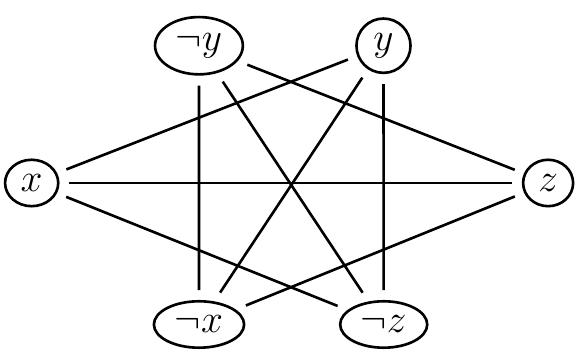
\includegraphics[width = 0.4\textwidth]{images/grafoCricca.png}
        \caption{Un grafo per l'espressione $(x \lor \neg y) \land (y \lor z) \land (\neg x \lor \neg z)$; l'insieme $\{\neg x, \neg y,z\}$ è una cricca di grado 3 e mostra come l'espressione sia soddisfacibile.}
        \label{fig:cricca}
    \end{figure}
\end{example}

\noindent Ci sono ancora un paio di problemi interessanti per gli sviluppi futuri.\
Per descriverli useremo una rappresentazione speciale delle funzioni booleane (totali) $f: \{\mathit{ff}, \mathit{tt}\}^n \rightarrow \{\mathit{ff}, \mathit{tt}\}$.\

Innanzitutto, dovrebbe già essere noto che tutte e sole le funzioni booleane sono rappresentabili da espressioni booleane; per i nostri scopi, basta dire che l'espressione booleana con $n$ variabili $B$ rappresenta $f(x_1, \dots ,x_n)$ quando dato l'assegnamento $\mathcal{V}(x_i) = t_i \in \{\mathit{ff},\mathit{tt}\}$,
\[f(x_1, \dots ,x_n)=\mathit{tt}\ \mbox{se e solamente se}\ \mathcal{V} \vDash B\]
Introduciamo adesso i circuiti booleani, che sono un altro modo ancora di rappresentare, o forse realizzare, le espressioni booleane e, per quanto detto, anche le funzioni booleane.

\begin{definition} [Circuito Booleano]
    Un \textit{circuito booleano} è un grafo diretto aciclico $(N,A)$, i cui nodi $1,\dots,n$ sono detti \textit{porte}, e i cui archi sono di solito rappresentati come coppie ordinate:\ un arco orientato da $i$ a $j$ è rappresentato da $(i, j)$.\

    Le porte hanno 0, 1, o 2 ingressi e sono di sorta $s(i) \in \{\mathit{tt},\mathit{ff},\neg, \land, \lor\} \cup X$, dove $X$ è l'insieme delle \textit{variabili};

    Gli \textit{ingressi} $i$ del circuito sono le porte di sorta $s(i) \in \{\mathit{tt},\mathit{ff}\} \cup X$, e non hanno ingressi; l'\textit{uscita} del circuito è, per convenzione, la porta $n$ senza uscite\footnote{La restrizione di avere una singola uscita si può facilmente rimuovere, permettendo così di avere circuiti con molte uscite.}; tutte le altre porte hanno un'uscita e quando $s(i) = \neg$, la porta $i$ ha un solo ingresso e quando $s(i) \in \{\land, \lor\}$, allora la porta $i$ ha 2 ingressi.

    Come visto prima, per rappresentare le funzioni booleane ci serve un assegnamento $\mathcal{V}$ di valori di verità alle variabili di un circuito $C$, che postuliamo essere buono, cioè tale da legare ogni variabile di $C$ a un valore in $\{\mathit{tt}, \mathit{ff}\}$.\

    Allora il valore di verità $[\![i]\!]_{\mathcal{V}}$ calcolato dalla porta $i$ è definito induttivamente dalle seguenti clausole:
    \begin{table}[H]
        \centering
        \begin{tabular}{l l l}
            $[\![i]\!]_\mathcal{V}$ & = $\mathit{tt}$                                       & se $s(i) =\mathit{tt}$                 \\
                                    & = $\mathit{ff}$                                       & se $s(i) =\mathit{ff}$                 \\
                                    & = $\mathcal{V}(x)$                                    & se $s(i) =x$                           \\
                                    & = not $[\![j]\!]_\mathcal{V}$                         & se $s(i) = \neg$ e $(j,i)\in A$        \\
                                    & = $[\![j]\!]_\mathcal{V}$ or $[\![k]\!]_\mathcal{V}$  & se $s(i) = \lor$ e $(j,i),(k,i)\in A$  \\
                                    & = $[\![j]\!]_\mathcal{V}$ and $[\![k]\!]_\mathcal{V}$ & se $s(i) = \land$ e $(j,i),(k,i)\in A$ \\
        \end{tabular}
    \end{table}
    \noindent Infine il valore del circuito è $\mathcal{V}(C) = [\![n]\!]_\mathcal{V}$, quello della porta di uscita.\
\end{definition}

\noindent Per comprendere meglio cos'è un circuito, consideriamo l'espressione booleana $(x \lor (x \land y)) \lor ((x \land y) \land \neg(y \lor z))$ che può essere espressa mediante circuito rappresentato in figura \ref{fig:circ}.

\begin{figure}[H]
    \centering
    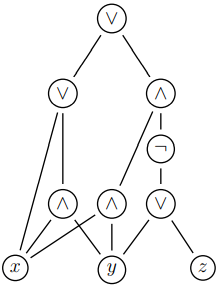
\includegraphics[scale=0.6]{images/Circuito.PNG}
    \caption{Un circuito booleano soddisfacibile.}
    \label{fig:circ}
\end{figure}

\noindent Possiamo ora descrivere un altro problema, e poi una sua variante, che verranno usati per caratterizzare le classi $\mathcal{P}$ e $\mathcal{NP}$.

\vspace{12pt}
\noindent\textbf{Problema CIRCUIT SAT}\quad Il problema {\footnotesize CIRCUIT SAT}, o della \textit{soddisfacibilità dei circuiti}, consiste nel decidere se esiste un assegnamento $\mathcal{V}$ tale che $\mathcal{V}(C)=\mathit{tt}$.\

\medskip
\noindent Un modo immediato per risolvere questo problema è di sostituire alle variabili $x, y, z,\dots$ \textit{tutte le possibili} combinazioni di $\mathit{tt}, \mathit{ff}$ e di \textit{controllare} una ad una le combinazioni per verificare se sono una soluzione.\
Questa è ancora una volta una ricerca esaustiva per forza bruta.\
La versione non deterministica mostra che $\mbox{\footnotesize CIRCUIT SAT} \in \mathcal{NP}$ e prevede due passi:\ nel primo si sceglie in tempo polinomiale non deterministico l'assegnamento ``giusto'' tra i $2^n$ possibili assegnamenti, se $n$ sono le variabili; nel secondo, \textit{polinomiale} nel numero delle porte del circuito, si \textit{certifica} il risultato.\
Questo secondo passo può essere opportunamente visto come un problema di decisione, visto che risulterà essere particolarmente interessante.\

\vspace{12pt}
\noindent\textbf{Problema CIRCUIT VALUE}\quad Il problema {\footnotesize CIRCUIT VALUE} consiste nel calcolare il valore di un circuito \textit{senza variabili}, ovvero in cui gli ingressi sono porte di sorta $s(i) \in \{\mathit{tt}, \mathit{ff}\}$.\

\medskip
\noindent È immediato vedere che questo problema appartiene a $\mathcal{P}$:\  basta ``arrampicarsi'' sull'ordinamento parziale a partire dalle porte di ingresso, valutando i valori di uscita delle $n$ porte livello per livello; non ci si faccia confondere dal fatto che il numero totale delle porte può essere esponenziale rispetto la profondità del circuito, cioè il livello della porta di uscita:\ la taglia del circuito è data infatti proprio dal numero $n$ delle sue porte.

Per calcolare il valore di un circuito è sufficiente allora al passo $i$-esimo memorizzare su un nastro di lavoro i valori delle porte di quel livello, usando i valori calcolati ai passi precedenti, ovvero quelli delle porte di livello inferiore, che sono stati via via memorizzati sul nastro di lavoro; i valori delle porte di ingresso stanno sul nastro di ingresso.\

\subsection{Problemi completi per P e NP}

Iniziamo con alcune proprietà che ci saranno utili per presentare alcuni problemi e poi dimostrarli completi per $\mathcal{P}$ ed $\mathcal{NP}$.\

Il seguente teorema è banale e illustra un tipo speciale di riduzione:\ quella per \textit{generalizzazione}.\
Ogni caso particolare di un problema si riduce al problema stesso nella sua piena generalità attraverso la funzione identità.

\begin{property}
    $\mbox{\footnotesize CIRCUIT VALUE} \leqslant_{\mathrm{logspace}} \mbox{\footnotesize CIRCUIT SAT}.$
\end{property}

\noindent Correliamo adesso {\footnotesize CIRCUIT SAT} a un problema appena più complesso e facciamo vedere che quando due problemi sono molto simili è facile trovare una riduzione tra essi (e chi l'avrebbe mai detto?); l'esempio che consideriamo è la riduzione di {\footnotesize CIRCUIT SAT} a {\footnotesize SAT}.

\begin{property}
    $\mbox{\footnotesize CIRCUIT SAT} \leqslant_{\mathrm{logspace}} \mbox{\footnotesize SAT}.$
    \label{CircuitSatSiRiduceASAT}
\end{property}

\begin{proof}

    Dato il circuito $C = (N,A)$ con variabili in $X$, dobbiamo trovare una riduzione $f \in \mathrm{LOGSPACE}$ tale che l'espressione booleana $f(C)$ sia soddisfacibile se e solamente se $C$ lo è, in simboli tale che se $\exists \mathcal{V}.\ [\![C]\!]_\mathcal{V} = \mathit{tt}$ allora e solamente allora $\exists \mathcal{V}'$ tale che $\forall x \in X.\ \mathcal{V}'(x) = \mathcal{V}(x) $ e $\mathcal{V}' \vDash f(C)$.\
    Il gioco è facile, perché sia i circuiti che le espressioni booleane rappresentano funzioni booleane, ma non è affatto banale.

    \begin{itemize}
        \item[i)] Le variabili $x$ di $f(C)$ sono quelle di $C$ unite a un nuovo insieme che contiene una nuova variabile per ogni porta di $C$; per semplicità, diamo a queste nuove variabili lo stesso nome che hanno le porte, fidandoci del fatto che il contesto ci dice quando sono le une e quando le altre;
        \item[ii)] per ogni porta $g$ di $C$ costruiamo i congiunti di $f(C)$ così:
              \begin{itemize}
                  \item se $g$ è la porta di uscita, allora genera il congiunto $g$; ciò garantisce che l'assegnamento $\mathcal{V}'$ manderà $g$ in $\mathit{tt}$ altrimenti l'intera formula $f(C)$ risulterebbe falsa;
                  \item se $s(g) = \mathit{tt}$ (o $\mathit{ff}$) allora genera $g$ (oppure $\neg g$), e l'equivalenza è ovvia --- si noti che se il circuito avesse solo una porta $g$ di sorta $\mathit{ff}$ la sua immagine sotto $f$ sarebbe $g \land \neg g$ che non può essere soddisfacibile (il primo congiunto viene dalla prima condizione, il secondo da quella che stiamo considerando);
                  \item se $s(g) = x \in X$ allora genera $(\neg g \lor x) \land (g \lor \neg x)$, ovvero $g \Longleftrightarrow x$ (cioè $g$ \textit{se e solamente se $x$}, ricordando la definizione di $\Longleftrightarrow$ in termini di $\neg, \lor$ e $\land$).\
                        Quindi entrambi i congiunti sono soddisfatti da $\mathcal{V}'(g) = \mathcal{V}'(x) = \mathcal{V}(x)$;
                  \item se $s(g) = \neg$ e $(h, g) \in A$ allora genera $(\neg g \lor \neg h) \land (g \lor h)$, ovvero $g \Longleftrightarrow \neg h$, e l'equivalenza tra le due formulazioni è ancora ovvia;
                  \item se $s(g) = \lor$ e $(h, g),(k, g) \in A$ allora genera $(\neg h \lor g) \land (\neg k \lor g) \land (h \lor k \lor \neg g)$, ovvero $g \Longleftrightarrow (h \lor k)$, e l'equivalenza tra le due formulazioni è immediata;
                  \item se $s(g) = \land$ e $(h, g),(k, g) \in A$ allora genera $(\neg g \lor h) \land (\neg g \lor k) \land (\neg h \lor \neg k \lor g)$, ovvero $g \Longleftrightarrow (h \land k)$, e l'equivalenza tra le due formulazioni è immediata ancora una volta.
              \end{itemize}
    \end{itemize}
    La dimostrazione che la trasformazione richiede spazio logaritmico si basa sulle stesse osservazioni fatte per mostrare che {\footnotesize HAM} si riduce a {\footnotesize SAT}.

\end{proof}

\begin{example}

    Per vedere come funziona la riduzione delineata nella dimostrazione precedente, si consideri il semplicissimo circuito illustrato in Figura \ref{fig:circuitEx}, composto da tre porte $g,h$ e $k$ con $g$ porta di uscita e $s(g) = \land$ e $h,k$ porte di ingresso di sorta rispettivamente $x$ e $\mathit{ff}$.\

    \begin{figure}[H]
        \centering
        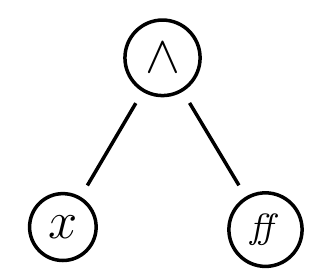
\includegraphics[width=0.2\textwidth]{images/CircuitoExample.png}
        \caption{}
        \label{fig:circuitEx}
    \end{figure}

    \noindent Naturalmente $C$ sempre ha valore $\mathit{ff}$ e quindi ci aspettiamo un'espressione $f(C)$ non soddisfacibile.\
    La porta di uscita genera i seguenti quattro congiunti, il primo per la prima condizione, gli altri tre per l'ultima:\ $g \land (g \lor \neg h \lor \neg k) \land (\neg g \lor h) \land (\neg g \lor k)$.\
    La porta $h$ genera i seguenti due congiunti:\ $(\neg h \lor x) \land (h \lor \neg x)$.\
    Infine la porta $k$ genera $\neg k$.\

    È immediato verificare che la congiunzione di tutte queste sette disgiunzioni non è soddisfacibile poiché a $g$ deve essere assegnato il valore $\mathit{tt}$ e quindi $(\neg g \lor k)$ valuta a $\mathit{tt}$ se e solamente se a $k$ viene assegnato il valore $\mathit{tt}$, ma in questo caso l'ultimo congiunto $\neg k$ varrebbe $\mathit{ff}$.
\end{example}

\noindent Solo per ricordare che la classe LOGSPACE è chiusa per composizione e transitività (vedi il teorema \ref{class_logspace}) possiamo enunciare anche le seguenti proprietà.

\begin{corollario}
    \hfill
    \begin{itemize}
        \itemsep0px
        \item[] $\mbox{\footnotesize CIRCUIT VALUE} \leqslant_{\mathrm{logspace}} \mbox{\footnotesize SAT}$
        \item[] $\mbox{\footnotesize CIRCUIT VALUE} \leqslant_{\mathrm{logspace}} \mbox{\footnotesize CRICCA}$
    \end{itemize}
\end{corollario}

\noindent Possiamo passare adesso a caratterizzare $\mathcal{P}$ e $\mathcal{NP}$ mediante uno o più problemi completi.\
Ricordiamo anche che, data una classe di funzioni $F$ tale che $\leqslant_F$ classifica $\mathcal{D}$ ed $\mathcal{E}$ (con $\mathcal{D} \subseteq\mathcal{E}$), se un problema $A$ è completo per $\mathcal{E}$ e $A \in \mathcal{D}$ allora $\mathcal{E} = \mathcal{D}$.\
Quindi studiare i problemi completi per una classe significa davvero caratterizzarla.\
Prima abbiamo po' di abbreviazioni e di ipotesi di lavoro, per semplificare le dimostrazioni e standardizzare la nozione di computazione.\
La più importante riguarda un modo di rappresentare le computazioni delle macchine deterministiche come una successione di configurazioni opportunamente organizzate in una matrice.\
La definizione copre il caso di macchine a 1 nastro, ma se la macchina fosse a $k$ nastri la potremmo sempre ridurre in tempo polinomiale a una macchina a 1 nastro grazie al teorema \ref{riduzione_nastri}, riportandoci al caso precedente.

\begin{definition} [Tabella di Computazione]

    La \textit{tabella di computazione} $T_M$ di una macchina di Turing $M$ a 1 nastro deterministica, o semplicemente $T$ quando non vi sia ambiguità, è una matrice quadrata il cui indice di riga $i$ rappresenta l'$i$-esimo passo di computazione e il cui indice di colonna $j$ rappresenta la $j$-esima posizione sul nastro.\
    Di conseguenza, la riga $i$-esima rappresenta la configurazione di $M$ dopo il passo $i-1$ e l'elemento $T(i,j)$ contiene il simbolo contenuto nella cella $j$-esima del nastro dopo $i-1$ passi di computazione.\

\end{definition}

\noindent Se $M$ decide il problema $I$ in tempo polinomiale deterministico $|x|^k$, la sua tabella di computazione (o semplicemente la sua computazione) su $x$ ha al massimo $|x|^k$ righe e altrettante colonne.\footnote{Con queste dimensioni, una tabella di computazione ha ovviamente abbastanza righe, ed ha anche abbastanza colonne, perché non si può usare più spazio che tempo.}

\medskip
\noindent Per semplificarci la vita, facciamo alcune ulteriori standardizzazioni.\
Data una macchina $M$, conveniamo che

\begin{enumerate}
    \item il valore di $k$ sia tale per cui la macchina $M$ si arresta prima di $|x|^k -2$ passi --- quindi $k$ deve essere abbastanza grande per garantirlo (v.\ anche il punto 5) e ciò è facile quando $|x| \geq 2$; se invece $|x| \leq 1$ allora agisci localmente su questo caso particolare, ovvero fai come se non esistesse.\
          (A dire il vero, sarebbe sufficiente considerare tabelle di dimensione $|x|^k + 2$, ma tale valore risulterebbe noioso da scrivere.)
    \item  Il nastro è riempito nelle posizioni non significative a destra con tanti \# quanti ne servono per arrivare alla casella in colonna $|x|^k$:\ la testina di $M$ non oltrepasserà mai tale posizione --- in una macchina che decide un problema, il tempo limita lo spazio!
    \item Arricchiamo l'alfabeto di $M$ in modo che la casella $T(i, j)$ contenga il nuovo simbolo $\sigma_q$, per registrare che nella configurazione $i$-esima la testina viene a trovarsi sulla $j$-esima casella, il simbolo letto è $\sigma$ e lo stato corrente è $q$ --- per far ciò basta prendere $\Sigma \times Q$ nuovi simboli, che sono la congiunzione del simbolo $\sigma$ e dello stato $q$.
    \item La configurazione iniziale ha la testina sul carattere immediatamente a destra del simbolo di inizio nastro, cioè $M$ inizia a calcolare da $\triangleright \underline{\sigma}_{q_0}w$ e non da $\underline{\triangleright}_{q_0}\sigma w$.\
          Inoltre trasformiamo la funzione di transizione di $M$ in modo che la testina non si posizioni mai sul simbolo di inizio stringa $\triangleright$ (quando ciò accadesse, basterebbe condensare in un solo passo i due compiuti dalla macchina $M$:\ lo spostamento a sinistra sulla casella contenente il simbolo $\triangleright$ e il successivo spostamento a destra).\
          Questa ipotesi fa sì che $\triangleright$ si comporti come un vero respingente!\ c'è però l'eccezione riportata nel punto seguente.
    \item Se $T(i, j) \in \{\sigma_{SI}, \sigma_{NO}\}$ allora ``sposta'' il cursore fino alla seconda colonna (con al massimo $\mathcal{O}\left(|x|^k\right)$ passi, introducendo uno stato ausiliario di finto arresto).\
          Cioè lo stato di accettazione, se è raggiunto, sia sempre in $T(l, 2)$ per qualche $l \leq |x|^k$.\
          Si noti che anche queste manovre possono influire sul valore di $k$, per esempio nel caso in cui $M$ si arresti proprio all'estremità destra del nastro.\
          Inoltre, come eccezione del punto precedente, si ammette che la testina si sposti sopra il simbolo $\triangleright$ quando lo stato sia $q_{SI}$ (abbreviazione di $\sigma_{q_{SI}}$), con il vincolo che non debba \textit{mai} toccare il simbolo $\triangleright$ più a sinistra, che rappresenta l'inizio del nastro (v.\ ipotesi 4).
    \item Se $\sigma_{SI}$ oppure $\sigma_{NO}$ appaiono sulla riga $p < |x|^k$ e nella seconda colonna, allora tutte le righe di indice $q$, $p \leq q \leq |x|^k$, sono uguali alla $p$-esima.
\end{enumerate}

\noindent Per finire, abbiamo l'ovvia condizione di terminazione con successo:\ $M$ accetta $x$ se e solamente se esiste $i$ tale che $T(i, 2) = \sigma_{SI} (= T(|x|^k, 2))$.\

\medskip
\noindent\textit{Osservazione}\quad Sia $M$ una macchina di Turing che decide $I$ in $|x|^k$, e $T$ la sua tabella di computazione su $x$.\
Abbiamo che

\begin{itemize}
    \item la cella $T(1,2)$ contiene lo stato iniziale e il primo carattere di $x$; inoltre $\forall j.\ 2 \leq j \leq |x|+1$, la casella $T(1,j)$ contiene il $(j-1)$-esimo simbolo di $x$; infine $\forall j\ |x| + 2 \leq j \leq |x|^k$, la cella $T(1,j)$ contiene \#;
    \item $\forall i.\ T(i,1) = \triangleright$;
    \item $\forall i.\ T\left(i,|x|^k\right) = \#$ --- si impiega meno spazio che tempo.
\end{itemize}

\noindent Quindi la prima riga è completamente determinata dal dato di ingresso e la prima e l'ultima colonna sono fisse in \textit{tutte} le tabelle di computazione.\

La cosa importante adesso è capire come si determina $T(i,j)$ in tutti gli altri casi, una volta fissata la funzione di transizione $\delta$; il suo valore \textit{dipende solo da tre caselle}:\ quelle della riga precedente, nella stessa posizione o in quelle immediatamente ai suoi lati, cioè \textit{il valore di} $T(i,j)$ \textit{è completamente determinato da quelli di} $T(i-1,j-1), T(i-1,j), T(i-1, j+1)$.\

\medskip
\noindent Per convincersene si esamini la figura \ref{fig:tabella} e si considerino i seguenti casi:

\begin{itemize}
    \item[i)] Se le tre caselle contengono $\sigma \in \Sigma$, cioè il cursore non si trova su alcune di esse, allora $T(i,j)= T(i-1,j)$.
    \item[ii)] Se una di esse contiene $\sigma_q$, cioè è la casella su cui c'è il cursore, allora $T(i,j)$, che può essere diverso da $T(i-1,j)$ per effetto di uno spostamento e/o di una scrittura, è completamente determinato da $\delta(\sigma, q)$ e quindi da $T(i-1,j-1), T(i-1,j)$ e $T(i-1,j+1)$.\
\end{itemize}

\begin{figure}[H]
    \centering
    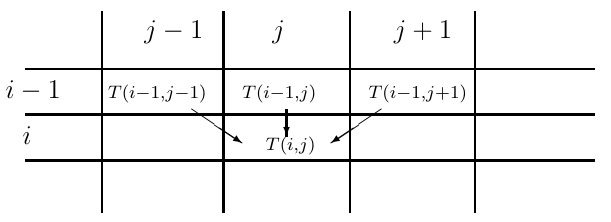
\includegraphics[width=0.6\textwidth]{tabellaComputazione}
    \caption{\textit{Le tre caselle nella riga $i - 1$ e nelle colonne $j - 1, j, j + 1$ (corrispondenti a quelle della configurazione precedente) determinano la casella $T(i, j)$ (corrispondente a quella della configurazione attuale).}}
    \label{fig:tabella}
\end{figure}

\subsubsection{$\mathcal{P}$-completezza}

Siamo pronti per presentare formalmente il primo problema $\mathcal{P}$-completo e a dimostrare che lo è davvero.

\begin{theorem}[{\footnotesize CIRCUIT-VALUE} è $\mathcal{P}$-completo]
    \label{CircVal_P-completo}
    \hfill

    {\footnotesize CIRCUIT-VALUE} è $\leqslant_{\mathit{logspace}}$-completo per $\mathcal{P}$.
\end{theorem}

\begin{proof}

    Sappiamo già che {\footnotesize CIRCUIT-VALUE} $\in \mathcal{P}$, quindi prendiamo un qualunque $I \in \mathcal{P}$ e facciamo vedere che c'è una riduzione $f \in$ LOGSPACE che lo trasforma in {\footnotesize CIRCUIT-VALUE}; ovvero $x \in I$ se e solamente se $f(x)$ è un circuito \textit{senza} variabili il cui valore è $\mathit{tt}$.\

    \medskip
    \noindent Sia $M$ una macchina di Turing che decide $I$ in $n^k$, e $T$ la sua tabella di computazione su $x$ e inoltre sia $\Sigma'$ l'alfabeto di $M$ unito ai nuovi simboli $\sigma_q \in \Sigma \times (Q \cup \{\epsilon\})$ che si usano per costruire la tabella $T$.\

    Come primo passo della dimostrazione costruiamo un circuito a partire dalla tabella di computazione di $M$.\
    Per far ciò codifichiamo ogni simbolo $\rho \in \Sigma'$ con una stringa di bit $(S_1,\dots,S_m) \in \{\mathit{tt},\mathit{ff}\}^m$, dove naturalmente $m = \lceil \log\#(\Sigma') \rceil$.\
    Con questa rappresentazione, la tabella di computazione $T$ risulta avere $|x|^k$ righe che sono stringhe di bit, ciascuna lunga $m \times |x|^k$.\
    Possiamo allora rappresentare ciascun elemento della tabella con $S_{i,j,l}$, con $1 \leq i,j \leq |x|^k$ e $l \leq m$.\

    Innanzitutto, $\forall i$ la $m$-upla $S_{i,1,1}\dots S_{i,1,m}$ codifica il simbolo $\triangleright$ e analogamente $\forall i.\ S_{i,|x|^k,1}\dots S_{i,|x|^k,m}$ codifica il simbolo $\#$.\

    Inoltre, poiché la funzione di transizione $\delta_M$ della macchina $M$ è fissata, possiamo usare l'osservazione fatta appena sopra riguardo al valore della casella $T(i,j)$ nella tabella di computazione:\ in modo del tutto analogo il valore di $S_{i,j,l}$ dipende solo dal valore delle tre sequenze di $m$ bit nella riga precedente con indice di colonna $j-1, j ,j+1$, cioè dai $3m$ bit $S_{i-1,j-1, l'}, S_{i-1,j,l''}, S_{i-1,j+1,l'''}$ con $1 \leq l', l'', l''' \leq m$.\
    Allora ci sono $m$ funzioni booleane $F_1, \dots, F_m$, con $3m$ ingressi ciascuna, tali che $\forall i,j >0$
    \[S_{i,j,l} = F_l = \left(
        \begin{array}{l l l}
                S_{i-1, j-1,1} & \dots & S_{i-1, j-1,m} \\
                S_{i-1, j,1}   & \dots & S_{i-1, j,m}   \\
                S_{i-1, j+1,1} & \dots & S_{i-1, j+1,m} \\
            \end{array}\right)\]
    A costo di essere noiosi ricordiamo che ciascuna funzione $F_l$ dipende \textit{solamente} dalla funzione di transizione $\delta_M$.\

    Adesso non è difficile costruire, seguendo lo stesso schema, una funzione che ``raggruppi'' $F_1,\dots,F_m$ in una sola funzione e che restituisca $m$ valori a fronte degli stessi $3m$ ingressi.\
    Per ogni funzione booleana, a uno o più valori, esiste un circuito, con lo stesso numero di uscite, che la calcola (come già accennato i circuiti booleani a $m$ valori hanno come porte di uscita $m$ porte, quelle senza archi uscenti).\
    Per ora abbiamo detto come costruire il circuito booleano $\overline{C}$ con $3m$ ingressi e $m$ uscite che codifica $T(i,j)$ dati $T(i-1,j-1), T(i-1,j)$ e $T(i-1,j+1)$; rappresentiamolo graficamente in figura \ref{fig:circ-dim}, dove abbiamo decorato ciascuna copia di $\overline{C}$ con gli indici $i$ e $j$ per rendere chiaro il suo legame con la casella $T(i,j)$; si confronti questa con la figura \ref{fig:circ}, osservando che nelle nostre rappresentazioni le computazioni ``procedono'' verso il basso, i segnali ``fluiscono'' verso l'alto.\
    A questo punto facciamo un'osservazione molto importante:\ poiché il circuito $\overline{C}$ dipende \textit{solo} dalla funzione di transizione $\delta_M$ di $M$, la sua taglia, comunque sia misurata, purché in modo ``ragionevole'', è \textit{fissata} ed è \textit{indipendente dall'input} $x$.
    \begin{figure}[H]
        \centering
        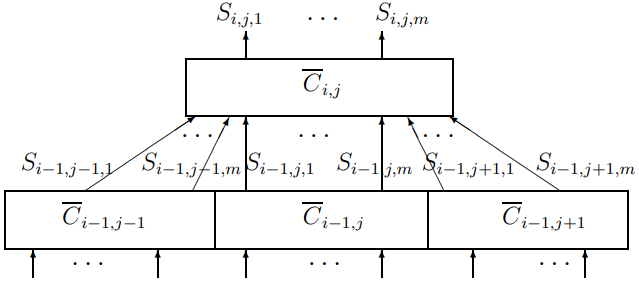
\includegraphics[width=0.6\textwidth]{images/circuitValue.PNG}
        \caption{Un circuito che calcola $T(i,j)$ dati $T(i-1,j-1), T(i-1,j)$ e $T(i-1,j+1)$.\ Ciascuno dei circuiti in basso ha $3\times m$ ingressi.}
        \label{fig:circ-dim}
    \end{figure}

    \noindent Siamo pronti per definire la riduzione $f$ da $I$ a {\footnotesize CIRCUIT-VALUE}.\
    Sostanzialmente, si tratta di trasformare la tabella della computazione $T$ in un circuito $C_I$, che è composto da una copia di $\overline{C}$ per ogni $T(i, j)$, come rozzamente illustrato illustrato in figura \ref{fig:circ-dim2}.\
    (Si noti che bastano $\left(|x|^k -1\right) \times \left(|x|^k-2\right)$ copie perché, grazie alle ipotesi fatte sulla forma della tabella di computazione, abbiamo fissato una volta per tutte la prima riga ($\forall j \geq 2.\ T(1,j) = \sigma_{j-1}$ se il dato d'ingresso è $\sigma_1, \dots, \sigma_{|x|}$) e la prima e l'ultima colonna ($\forall i \geq 1.\ T(i,1) = \triangleright$ e $T\left(i, |x|^k\right) = \#$, perché la prima macchina si arresta prima di $|x|^k -2$ passi).\ Quindi non c'è bisogno di costruire tali copie del circuito corrispondenti a tale riga e a tali colonne:\ basta prenderle dallo scaffale.)\
    Le uscite di $\overline{C}_{i-1, j-1},\overline{C}_{i-1, j},\overline{C}_{i-1, j+1}$ sono gli ingressi di $\overline{C}_{ij}$.\
    Gli ingressi di $C_I$ sono quelli di $T(1,j)$, $T(i,1), T\left(i, |x|^k\right)$, che sono determinati da $x$ o sono fissi.\
    Rappresentiamo adesso i simboli $\sigma_{SI}$ e $\sigma_{NO}$ corrispondenti all'accettazione o al rifiuto con stringhe composte rispettivamente da soli $\mathit{tt}$ e da soli $\mathit{ff}$.\
    Allora, l'uscita di $C_I$ è una delle uscite di $\overline{C}_{|x|^k, 2}$, poiché abbiamo convenuto che tali simboli appaiono sempre in posizione $T\left(|x|^k,2\right)$ (cf.\ l'ultima ipotesi fatta sulla tabella $T$).\

    \begin{figure}[H]
        \centering
        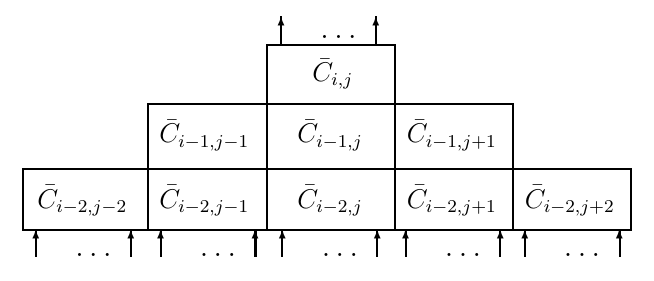
\includegraphics[width=0.6\textwidth]{images/circuitValue2.PNG}
        \caption{\textit{Una parte del circuito $C_I$, composto dal alcune copie di $\overline{C}$.}}
        \label{fig:circ-dim2}
    \end{figure}

    \noindent Il prossimo passo consiste nel verificare che $C_I = f(x)$ ha valore $\mathit{tt}$ se e solamente se $x \in I$.\
    Prima di tutto ricordiamo che le uscite di $\overline{C}_{i,j}$ rappresentano in binario il valore della cella $T(i, j)$ della tabella della computazione di $M$ su $x$.\ Delineiamo la dimostrazione che procede per induzione sul numero $i$ dei passi della computazione (indice di riga di $T$).\

    Se $i = 1$ banale.\
    L'ipotesi induttiva è che il valore per $i-1$ sia ben calcolato (e dipenda solo dai tre precedenti), cioè che $\forall j.\ \overline{C}_{i-1,j}$ ha come uscite $R_1,\dots, R_m$ se e solamente se $T(i-1,j) = \rho'$ e $\rho' \in \Sigma'$ è codificato proprio come $R_1,\dots, R_m$.\
    Dobbiamo dimostrare che $\overline{C}_{i,j}$ ha come uscite $S_1 \dots S_m$ se e solamente se $T(i,j) = \rho$, la cui codifica è $S_1 \dots S_m$.\
    Le uscite $S_1 \dots S_m$ sono state calcolate a partire da quelle di $\overline{C}_{i-1,j-1},\overline{C}_{i-1,j}$ e $\overline{C}_{i-1,j+1}$ in pieno accordo con la funzione di transizione $\delta_M$ di $M$, esattamente allo stesso modo in cui il valore di $T(i,j)$ lo è stato in funzione dei valori di $T(i-1,j-1),T(i-1,j)$ e $T(i-1,j+1)$.\
    Allora basta applicare l'ipotesi induttiva.\

    A questo punto è immediato dedurre che $\overline{C}_{|x|^k,2} = \mathit{tt}\dots \mathit{tt}$ se e solamente se $T(n^k, 2) = \sigma_{SI}$, ovvero $x \in I$ se e solamente se $f(x) = \mathit{tt}\dots\mathit{tt}$; analogamente per il caso $\overline{C}_{|x|^k, 2} = \mathit{ff}\dots\mathit{ff}$ e $\sigma_{NO}$.

    \medskip
    \noindent Vediamo infine che $f \in$ LOGSPACE, cioè che la riduzione può essere calcolata in spazio $\mathcal{O}(\log|x|)$, stimando lo spazio necessario ai nastri di lavoro.\
    Per calcolare $f$ dobbiamo costruire e connettere opportunamente tra loro
    \begin{itemize}
        \item[i)] le porte di ingresso --- facile, esamina $x$ e conta fino a $|x|^k$, ricordandosi $k$ in base 2 su un nastro di lavoro, scrivendo la codifica di $x$ (e di \# finché serve);
        \item[ii)] gli elementi della prima e dell'ultima colonna che sono $2 \times |x|^k$ circuiti costanti;
        \item[iii)] $\left(|x|^k - 1\right) \times \left(|x|^k - 2\right)$ copie del circuito $\overline{C}$ (che dipende, ricordiamolo, solo da $M$ e ha costo \textit{fisso}).\ A ciascuna copia associamo gli indici appropriati per metterla in relazione con la casella di computazione corrispondente; tali indici sono tutti minori di $|x|^k$, e averli rappresentati in binario ci consente di manipolarli in spazio $\mathcal{O}(\log(n))$.
    \end{itemize}

\end{proof}

\noindent Ritorniamo adesso rapidamente sulla distinzione tra approcci hardware e software ai modelli di calcolo fatta nel capitolo 1.5.\
Per quelli hardware, si suggeriva di vedere ciascun algoritmo come una macchina, le cui dimensioni potevano addirittura crescere al crescere dei dati di ingresso.\
Tale osservazione trova giustificazione nel circuito $C_I$ costruito nella dimostrazione precedente:\ al crescere del dato $x$ cresce la tabella di computazione della macchina di Turing $M$ e così crescono le \textit{dimensioni} del circuito corrispondente, ma non cambiano i suoi componenti $\overline{C}$ --- né cambia, per così dire, la sua forma.\

\medskip
\noindent Vediamo adesso una variante di {\footnotesize CIRCUIT-VALUE}, chiamato {\footnotesize MONOTONE CIRCUIT VALUE}:\ il problema di verificare se un circuito \textit{senza} $\neg$ calcola il valore $tt$.\
Si sa bene che le espressioni booleane e quindi i circuiti con soli $\land, \lor$ sono meno espressivi di quelli che hanno anche il $\neg$, tuttavia \textit{la difficoltà nel valutare gli uni e gli altri è la stessa}!\
Infatti non è difficile costruire una riduzione facile da {\footnotesize CIRCUIT-VALUE} a {\footnotesize MONOTONE CIRCUIT VALUE}.\

\begin{corollario}
    {\footnotesize MONOTONE CIRCUIT VALUE} è $\mathcal{P}$-completo.
\end{corollario}

\begin{proof}

    Facciamo vedere che {\footnotesize CIRCUIT-VALUE} $\leqslant_{\mathrm{logspace}}$ {\footnotesize MONOTONE CIRCUIT VALUE}, cioè trasformiamo un circuito qualunque (con ingressi assegnati) in uno monotono equivalente.\
    Ciò viene fatto applicando le regole di De Morgan partendo dalle porte di uscita a scendere fino alle porte di ingresso.\
    Le porte di ingresso $\mathit{tt}$ rimpiazzano se necessario quelle $\mathit{ff}$ e viceversa, e se ne aggiungono di nuove se servissero.\
    Tutto questo si fa ovviamente in LOGSPACE:\ basta visitare una sola volta le porte, rappresentate come coppie $(i, j)$, dove $i$ e $j$ sono indici di livello e di ``colonna'', rappresentati a loro volta in binario.

\end{proof}

\noindent Ecco un paio di problemi $\mathcal{P}$-completi, l'uno preso dalla teoria dei linguaggi formali e l'altro dalla logica; poiché appartengono allo stesso grado, vi sono trasformazioni sia dall'uno all'altro che da e in ({\footnotesize MONOTONE}) {\footnotesize CIRCUIT VALUE}.

\begin{example}
    \hfill
    \begin{itemize}
        \item $CFL \neq \emptyset$ è il problema di verificare se il linguaggio generato da una data grammatica libera da contesto\footnote{Una \textit{grammatica libera} è una quadrupla $G = \langle N, \Sigma, S, P\rangle$ dove $N$ è l'alfabeto dei simboli \textit{non terminali}, $\Sigma$ è l'alfabeto dei simboli \textit{terminali}, $S \in N$ è chiamato simbolo \textit{distinto}, $P \subseteq (N \times (N \cup \Sigma)^+)$ è l'insieme \textit{finito} delle \textit{produzioni}, usualmente rappresentate come $A \rightarrow \alpha$.} è vuoto, cioè:\ \[\{L(G) \neq \emptyset \mid G\ \mbox{è una grammatica libera dal contesto}\}\]
        \item dato un insieme di variabili $X$ e una congiunzione di un numero finito di formule di Horn \texttt{H},\footnote{Una formula booleana è un'espressione booleana nella forma \[x_1 \land x_2 \land \dots \land x_k \Longrightarrow y,\ y,x_i \in X,\ i \geq 0\] Inoltre, diciamo che $x$ è deducibile da una congiunzione di formule di Horn \texttt{H}, in simboli $\mathtt{H}\vdash x$, se e solamente se $x \in \mathtt{H}$ oppure $x_1 \land x_2 \land \dots \land x_k \Longrightarrow x$ e $ \forall i.\ \mathtt{H} \vdash x_i$} {\footnotesize HORN} è il problema di decidere se una variabile $x \in X$ è deducibile da \texttt{H}, cioè \[\mbox{\footnotesize HORN} = \{\mathtt{H}, x \mid \mathtt{H} \vdash x\}\]
    \end{itemize}
\end{example}

\newpage

\subsubsection{$\mathcal{NP}$-completezza}

Finalmente veniamo ai problemi intrattabili $\mathcal{NP}$ e al suo massimo campione, {\footnotesize SAT}, il problema della soddisfacibilità delle espressioni booleane.

\begin{theorem} [Cook]
    {\footnotesize SAT} è $\mathcal{NP}$-completo.
\end{theorem}

\begin{proof}

    Sappiamo già che {\footnotesize SAT} $\in \mathcal{NP}$, perché abbiamo visto una procedura non deterministica che realizza una ricerca esaustiva, seppur implicita e lo decide:\ assegna \textit{a caso} un valore di verità alle variabili dell'espressione booleana (fase che richiede tempo \textit{non deterministico} polinomiale) e valuta l'espressione (o il circuito) booleano chiuso che si ottiene (fase che richiede tempo \textit{deterministico} polinomiale); il problema è risolto positivamente se esiste un'espressione chiusa che valuta a $\mathit{tt}$.\

    Poiché {\footnotesize CIRCUIT-SAT} $\leqslant_{\mathrm{logspace}}$ {\footnotesize SAT} per la proprietà \ref{CircuitSatSiRiduceASAT}, ci basta dimostrare che {\footnotesize CIRCUIT-SAT} è $\mathcal{NP}$-completo, ovvero che $\forall I \in \mathcal{NP}$ si ha che $I \leqslant_{\mathrm{logspace}} \mbox{\footnotesize CIRCUIT-SAT}$.

    Sia allora $I \in \mathcal{NP}$.\
    Costruiamo $f \in$ LOGSPACE tale che $x \in I$ se e solamente se $f(x)$ è soddisfacibile.\
    Per ipotesi c'è una macchina di Turing non deterministica $N$ che decide $I$ in tempo $n^k$.\
    In altri termini, dato $x$ esiste una computazione di lunghezza minore o uguale a $|x|^k$ che accetta $x$ se e solamente se $x \in I$; ora, questa computazione può essere vista come una successione di scelte non deterministiche, anch'essa di lunghezza minore o uguale a $|x|^k$.\
    Per semplicità conveniamo che il grado di non determinismo sia \textit{esattamente} uguale a 2, cioè che ad ogni passo vi siano sempre 2 scelte possibili.\footnote{Possiamo sempre ricondurci a questa situazione:\ se la macchina $N$ ha
        \begin{itemize}
            \item[i)] solo una scelta, consideriamo due scelte coincidenti, il che richiede uno stato ausiliario;
            \item[ii)] $m > 2$ scelte, si sceglie la prima o le rimanenti $m-1$ e si ripete il procedimento $m-2$ volte, il che richiede di aggiungere $m-2$ nuovi stati.
        \end{itemize}}
    Codifichiamo la prima scelta con il bit $\mathit{ff}$ e la seconda con il bit $\mathit{tt}$.\
    Una computazione è allora una successione di bit della forma
    \[B = b_0 b_1 \dots b_{|x|^k-1},\ \mathrm{con}\ b_i \in \{\mathit{tt},\mathit{ff}\}\]
    Ovviamente nel caso della macchina non deterministica non abbiamo una tabella della computazione che rappresenti l'albero della computazione non-deterministica; tuttavia, se fissiamo una successione di scelte $B$ sappiamo costruire la tabella $T$ in funzione della macchina $N$, del dato $x$ e anche della successione di scelte $B$.\
    Quindi come fatto per {\footnotesize CIRCUIT-VALUE}, la prima riga e la prima e ultima colonna sono fissate.\
    Inoltre, $T(i,j)$ dipende, oltre che da $T(i-1,j-1), T(i-1,j)$ e $T(i-1,j+1)$ \textit{anche} da $b_{i-1}$, cioè dalla scelta fatta al passo precedente.\
    Quindi il circuito $\overline{C}_N$ che possiamo costruire in perfetta analogia a quanto fatto nella dimostrazione della $\mathcal{P}$-completezza di {\footnotesize CIRCUIT VALUE} (teorema \ref{CircVal_P-completo}), ha $3m + 1$ ingressi e $m$ uscite.\
    Di nuovo possiamo costruire in LOGSPACE un circuito $f(x)$ che ha come porte di ingresso le scelte non deterministiche codificate nel vettore $B$ e i valori della riga $T(1, j)$ ottenuti dal dato di ingresso $x$.\

    Infine, la dimostrazione che $f(x)$ è soddisfacibile se e solamente se $x \in I$ è del tutto simile a quella del teorema \ref{CircVal_P-completo}.

\end{proof}

\noindent Vediamo alcuni esempi di altri problemi che sono $\mathcal{NP}$-completi, cioè tali per cui vi sono trasformazioni dall'uno all'altro e da e in {\footnotesize SAT}.\
La letteratura riporta migliaia di problemi di questo tipo, la gran parte dei quali è significativa dal punto di vista computazionale --- quindi la classe $\mathcal{NP}$ è importante.

\begin{example}
    I seguenti problemi sono $\leqslant_{\mathrm{logspace}}$-completi per $\mathcal{NP}$.
    \begin{itemize}
        \item {\footnotesize HAM};
        \item {\footnotesize CRICCA};
        \item Problema del Commesso Viaggiatore;
        \item Programmazione Intera:\ dato un sistema di disequazioni a coefficienti interi in $n$ variabili trovare una soluzione intera.\footnote{Si ricordi che se si tralascia la parola ``intero'' il problema è in $\mathcal{P}$:\ basta usare il metodo elissoide o quello dei punti interni.}
    \end{itemize}
\end{example}

